\documentclass{beamer}
\beamertemplatenavigationsymbolsempty
\usecolortheme{beaver}
\setbeamertemplate{blocks}[rounded=true, shadow=true]
\setbeamertemplate{footline}[page number]
%
\usepackage[utf8]{inputenc}
\usepackage[english,russian]{babel}
\usepackage{amssymb,amsfonts,amsmath,mathtext}
\usepackage[]{algorithmic}
\usepackage{subfig}
\usepackage[all]{xy} % xy package for diagrams
\usepackage{array}
\usepackage{multicol}% many columns in slide
\usepackage{hyperref}% urls
\usepackage{hhline}%tables
% Your figures are here:
\graphicspath{ {fig/} {../fig/} }

%----------------------------------------------------------------------------------------------------------
\title[\hbox to 56mm{Петли скрытой обратной связи}]{ Условия существования петель скрытой \\ обратной связи в рекомендательных системах }
\author[А.\,А. Пилькевич]{Антон Александрович Пилькевич}
\institute{Московский физико-технический институт}
\date{\footnotesize
\par\smallskip\emph{Курс:} Автоматизация научных исследований\par (практика, В.\,В.~Стрижов)/Группа 813
\par\smallskip\emph{Эксперт:} А.\,С.~Хританков
\par\smallskip\emph{Консультант:} А.\,С.~Хританков
\par\bigskip\small 2021}
%----------------------------------------------------------------------------------------------------------
\begin{document}
%----------------------------------------------------------------------------------------------------------
\begin{frame}
\thispagestyle{empty}
\maketitle
\end{frame}
%-----------------------------------------------------------------------------------------------------
\begin{frame}{Цель исследования}
\begin{block}{Цель}
  Исследование условий существования петель обратной
связи в рекоммендательной системе с алгоритмом Thomson Sampling в условиях зашумлённости выбора пользователя.
\end{block}
\begin{block}{Задача}
  Нахождение математического описания условий возникновения петель и экспериментальная их проверка. 
\end{block}
\begin{block}{Решение}
  Усреденение смещение интереса и анализ зависимости от параметров шума. 
  Моделирование рекомендательной системы и поведения пользователя.
\end{block}
\end{frame}
%-----------------------------------------------------------------------------------------------------
\begin{frame}{Петли при параметрах шума $w, Q$}

Распределение отклика $c_t^i$ для рекомендации $\mathbf{a_t}$:
\begin{gather*}
    c_t^i \sim \text{Bern} \left(\sigma\left(\mu_t^i (a_t^i) + \mathbin{\color{red} q_t^i } \right) \right), \\ 
    \mu_{t+1} - \mu_{t} = \delta_t c_t - \delta_t (1 - c_t), 
\end{gather*}
где $q_t^i \sim \text{U}[-w, w], \delta_t \sim U[0, 0.01].$

\begin{columns}[c]
\column{0.3\textwidth}
Определение петель: 
\begin{gather*}
  \color{red} \lim_{t \to \infty} \|\mu_t - \mu_0 \|_2 = \infty.
\end{gather*}
\column{0.7\textwidth}
\begin{center}
  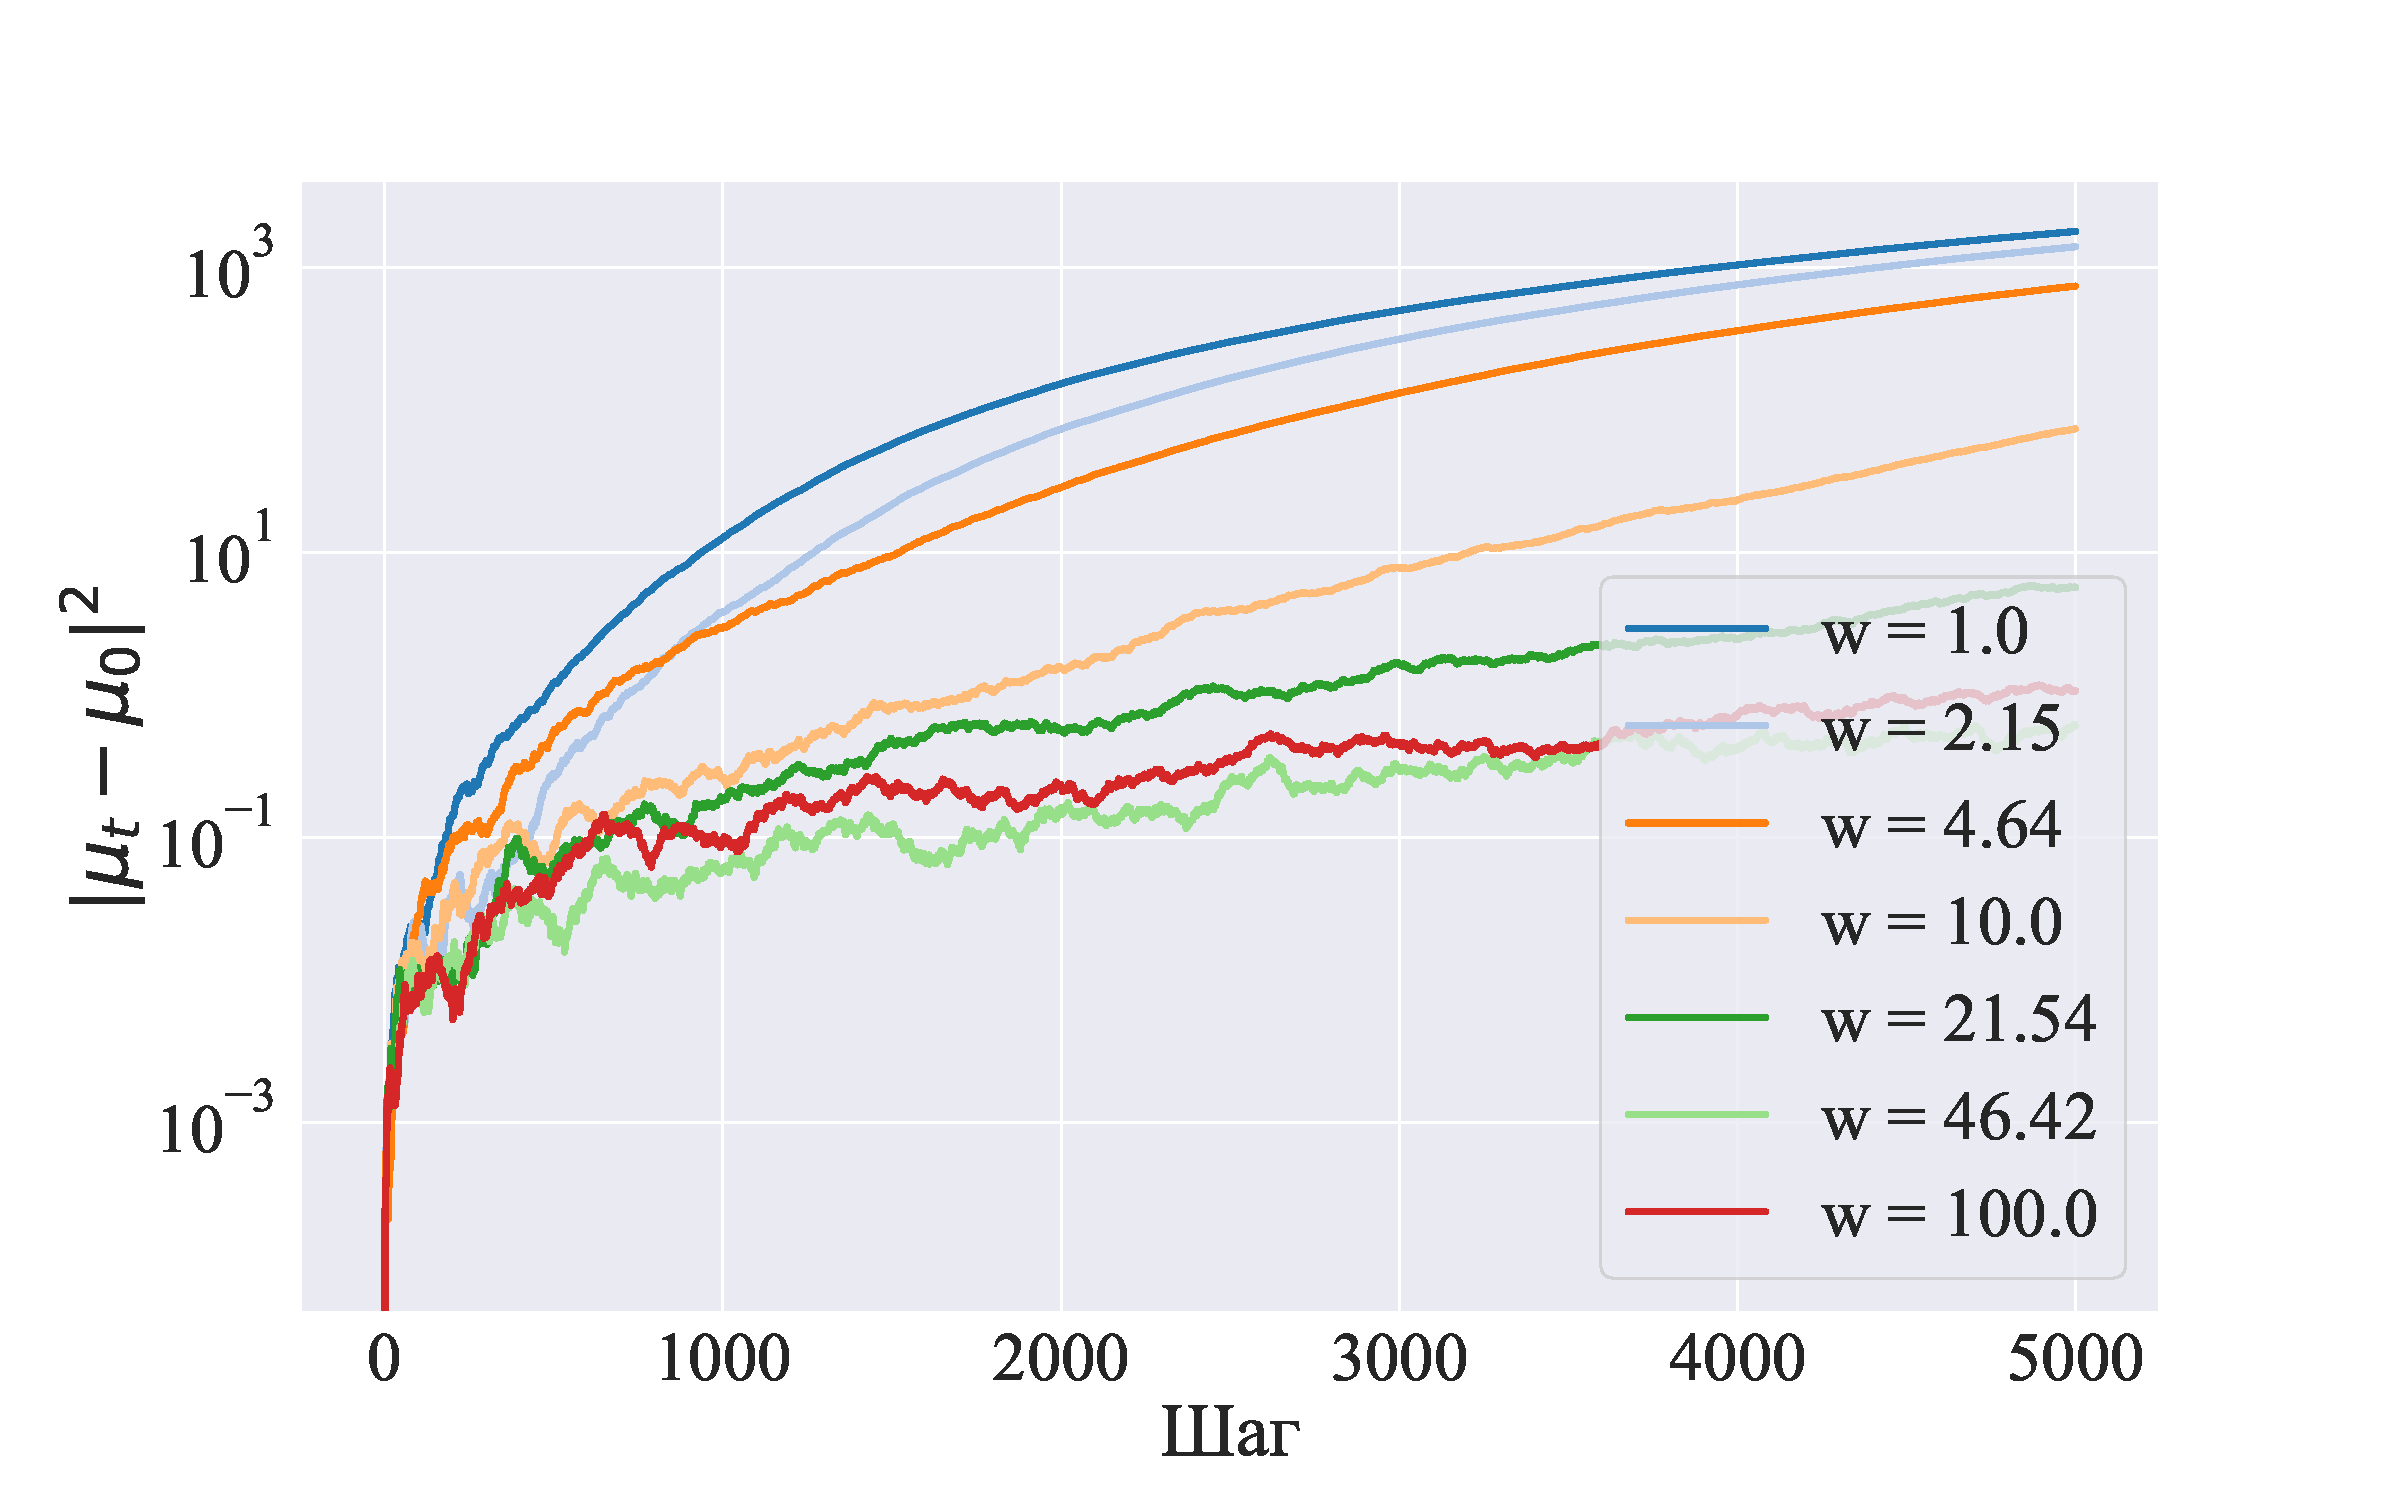
\includegraphics[width=7cm]{../norm_interest.pdf}
\end{center}
\end{columns}
\end{frame}


%----------------------------------------------------------------------------------------------------------
\begin{frame}{Публикации по теме}
\begin{enumerate}
    \item
      \textcolor{black}{Ray~Jiang, Silvia~Chiappa, Tor~Lattimore,Andr{\'a}s Gy{\"o}rgy, Pushmeet~Kohli.}
      \textcolor{blue}{Degenerate Feedback Loops in Recommender Systems}.
    \BibJournal{CoRR}, 2019, Vol. abs/1902.10730,
	  URL: \BibUrl{https://arxiv.org/abs/1902.10730}.

  \item
    \textcolor{black}{Khritankov, Anton.}
    \textcolor{blue}{Hidden Feedback Loops in Machine Learning Systems: A simulation Model and Preliminary Results}//
    \BibJournal{Springer}, 2021, P.~54--65.

  \item
    \textcolor{black}{Daniel Russo, Benjamin Van Roy, Abbas Kazerouni, Ian Osband.}
    \textcolor{blue}{A Tutorial on Thompson Sampling}//
    \BibJournal{CoRR}, 2017, Vol. abs/1707.02038,
	  URL: \BibUrl{https://arxiv.org/abs/1707.02038}.

  \item
    \textcolor{black}{Shipra Agrawal, Navin Goyal.}
    \textcolor{blue}{Analysis of Thompson Sampling for the multi-armed}//
    \BibJournal{CoRR}, 2011, Vol. abs/1111.1797,
	  URL: \BibUrl{https://arxiv.org/abs/1111.1797}.
  \end{enumerate}
\end{frame}
%----------------------------------------------------------------------------------------------------------
\begin{frame}{Модель данных}
  \begin{block}{Параметры}
  Множество объектов $M$, рекомендации $(a^1, \dots, a^l) \in M$, кол-во выдач $T$.
  Задаётся ф-ия описывающая интерес пользователя  в начальный момент времени $\mu_0 : M \to \mathbb{R}$.
\bigskip
\end{block}

\begin{columns}[T]
\column{0.5\textwidth}
\textcolor{blue}{Распределениее откликов:}   
\begin{gather*}
    c_t^i \sim \text{Bern} \left(\sigma\left(\mu_t^i (a_t^i) + \mathbin{\color{red} q_t^i } \right) \right), \\ 
    q_t^i \sim U[-w, w].
  \end{gather*}
\column{0.5\textwidth}
\textcolor{blue}{Эволюция интереса:}   
  \begin{gather*}
\mu_{t+1} - \mu_{t} = \delta_t c_t - \delta_t (1 - c_t), \\
\delta_t \sim U[0, 0.01].
  \end{gather*}
\end{columns}

\bigskip
\textcolor{blue}{Определение петли}:
\begin{gather*}
  \color{red} \lim_{t \to \infty} \|\mu_t - \mu_0 \|_2 = \infty.
\end{gather*}
\end{frame}
%----------------------------------------------------------------------------------------------------------
\begin{frame}{Thompson Sampling}
Априорное распределение для параметров интереса: 
\[Beta(1, 1) = U[0, 1].\] 
Апостериорное распределение для элемента $a^i \in M$ описывается $Beta(\alpha_t^i, \beta_t^i)$. 
Параметры обновляются по закону:
\[\alpha_{t+1} = \alpha_t + c_t, \beta_{t+1} = \beta_t + 1 - c_t.\]
Задача оптимизации бандита:
\begin{gather*}  
\max_{c_t^i} \sum_{t = 1}^T \sum_{i = 1}^l c_t^i = T \cdot l.\\ 
   T \cdot l - \sum_{t = 1}^T \sum_{i = 1}^l c_t^i \to \min_{b}, 
\end{gather*}
\end{frame}
%----------------------------------------------------------------------------------------------------------
\begin{frame}{Возникновение петли}
Назовём \textit{режимом работы TS с фиксированными лидерами} поведение алгоритма, в котором TS не меняются элементы рекомендаций.
  \begin{block}{Утверждение}
  Пусть  TS работает в режиме c фиксированными лидереми начиная с какого-то момента времени $\tau$ и используется аддитивная модель шума. 
  \end{block}
  \begin{block}{Анализ}
  \begin{itemize}
      \item Любой несмещённый аддитивный шум не влияет на возникновение петли. 
      \item При достаточно большом значение $\mu_t$ из-за $\sigma (x)$ шум $w$ перестаёт сколько-то значимо изменять истинный интерес. 
  \end{itemize}
  \end{block}
\end{frame}
%----------------------------------------------------------------------------------------------------------
\begin{frame}{Вычислительный эксперимент}
\begin{block}{Цель}
Проверка гипотезы о возникновении петель при параметрах шума, найденных из теоретических соотношений. 
\end{block}

\begin{block}{Алгоритм}
\begin{algorithmic}
  \REQUIRE{M, l, T, w, p}
  \STATE BanditLoopExperiment.prepare()
  \FOR{$t$ от $1$ до $T$} 
    \STATE $r_t \leftarrow$ TSBandit.predict()
    \STATE $c_t \leftarrow$ make\_response\_noise($r_t$, w, p)
    \STATE TSBandit.update($c_t$)
    \STATE Model.interest\_update($c_t$)
    \STATE save\_iter($t, c_t, \mu_t$)
  \ENDFOR
\end{algorithmic}
\end{block}

\end{frame}
%----------------------------------------------------------------------------------------------------------
\begin{frame}{Вычислительный эксперимент}
\begin{columns}[c]
\column{0.5\textwidth}
Зависимость нормы интeреса от итерации.
\begin{center}
  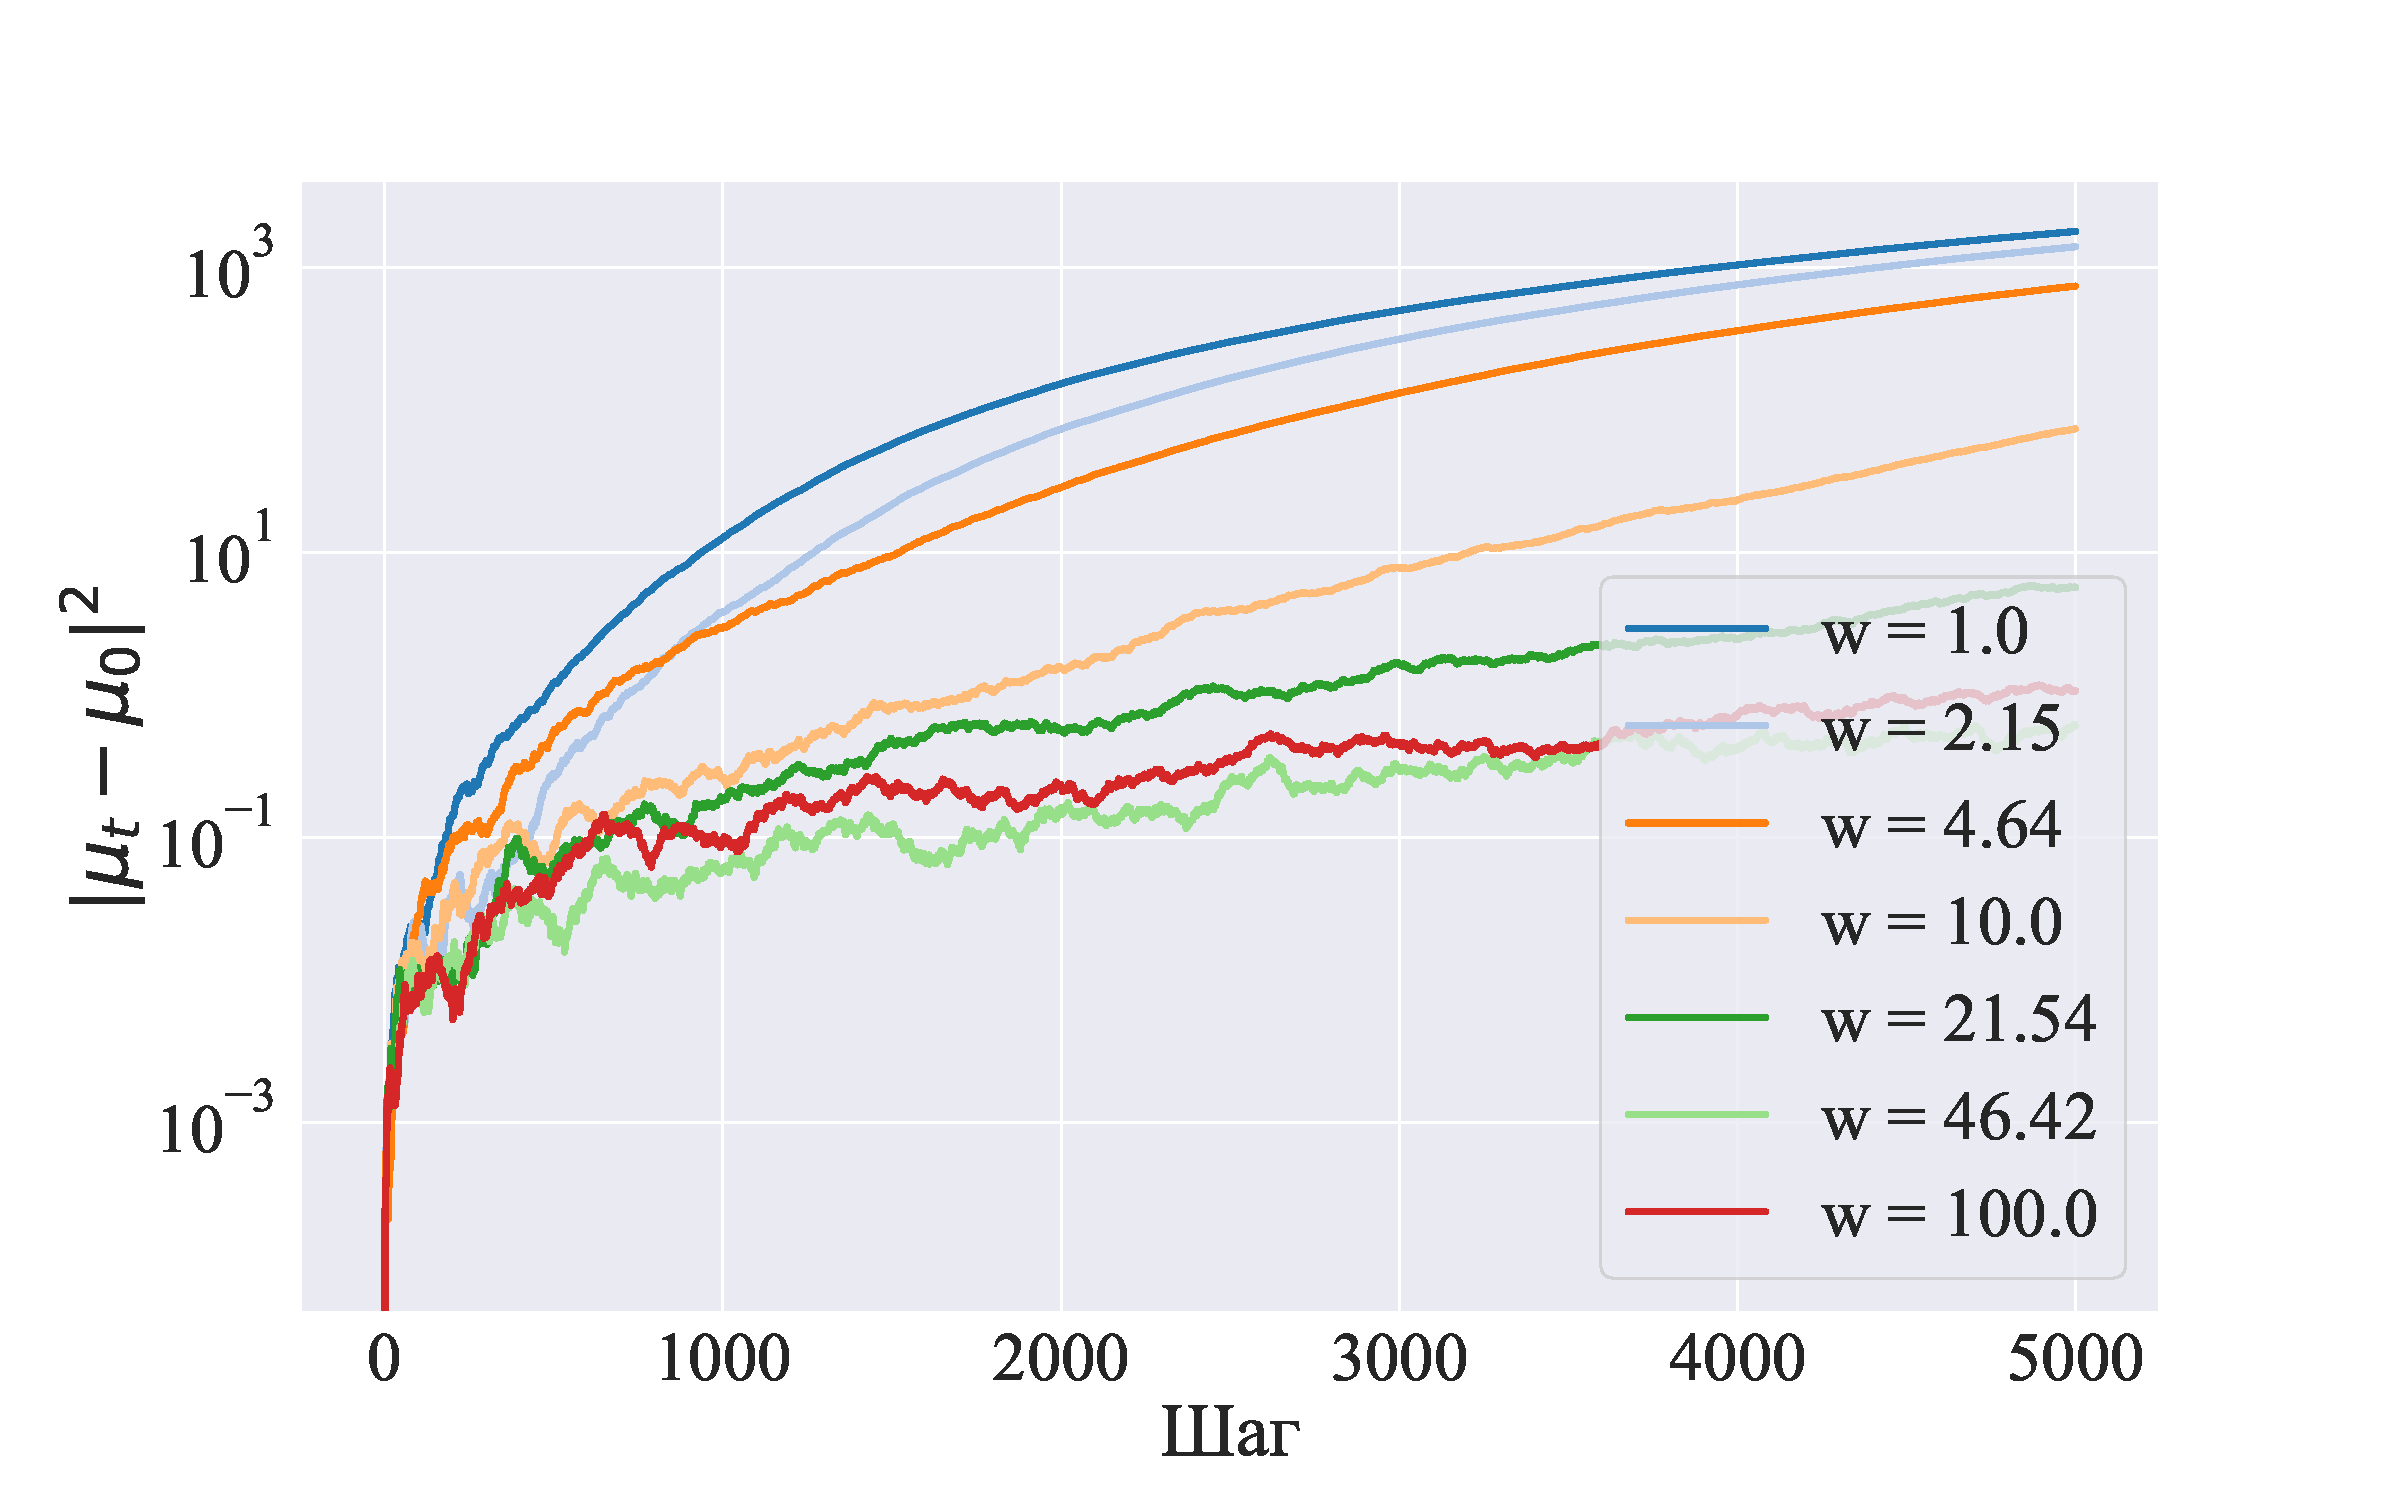
\includegraphics[width=6cm]{../norm_interest.pdf}
\end{center}
\column{0.5\textwidth}
Зависимость суммы откликов от итерации.  
\begin{center}
  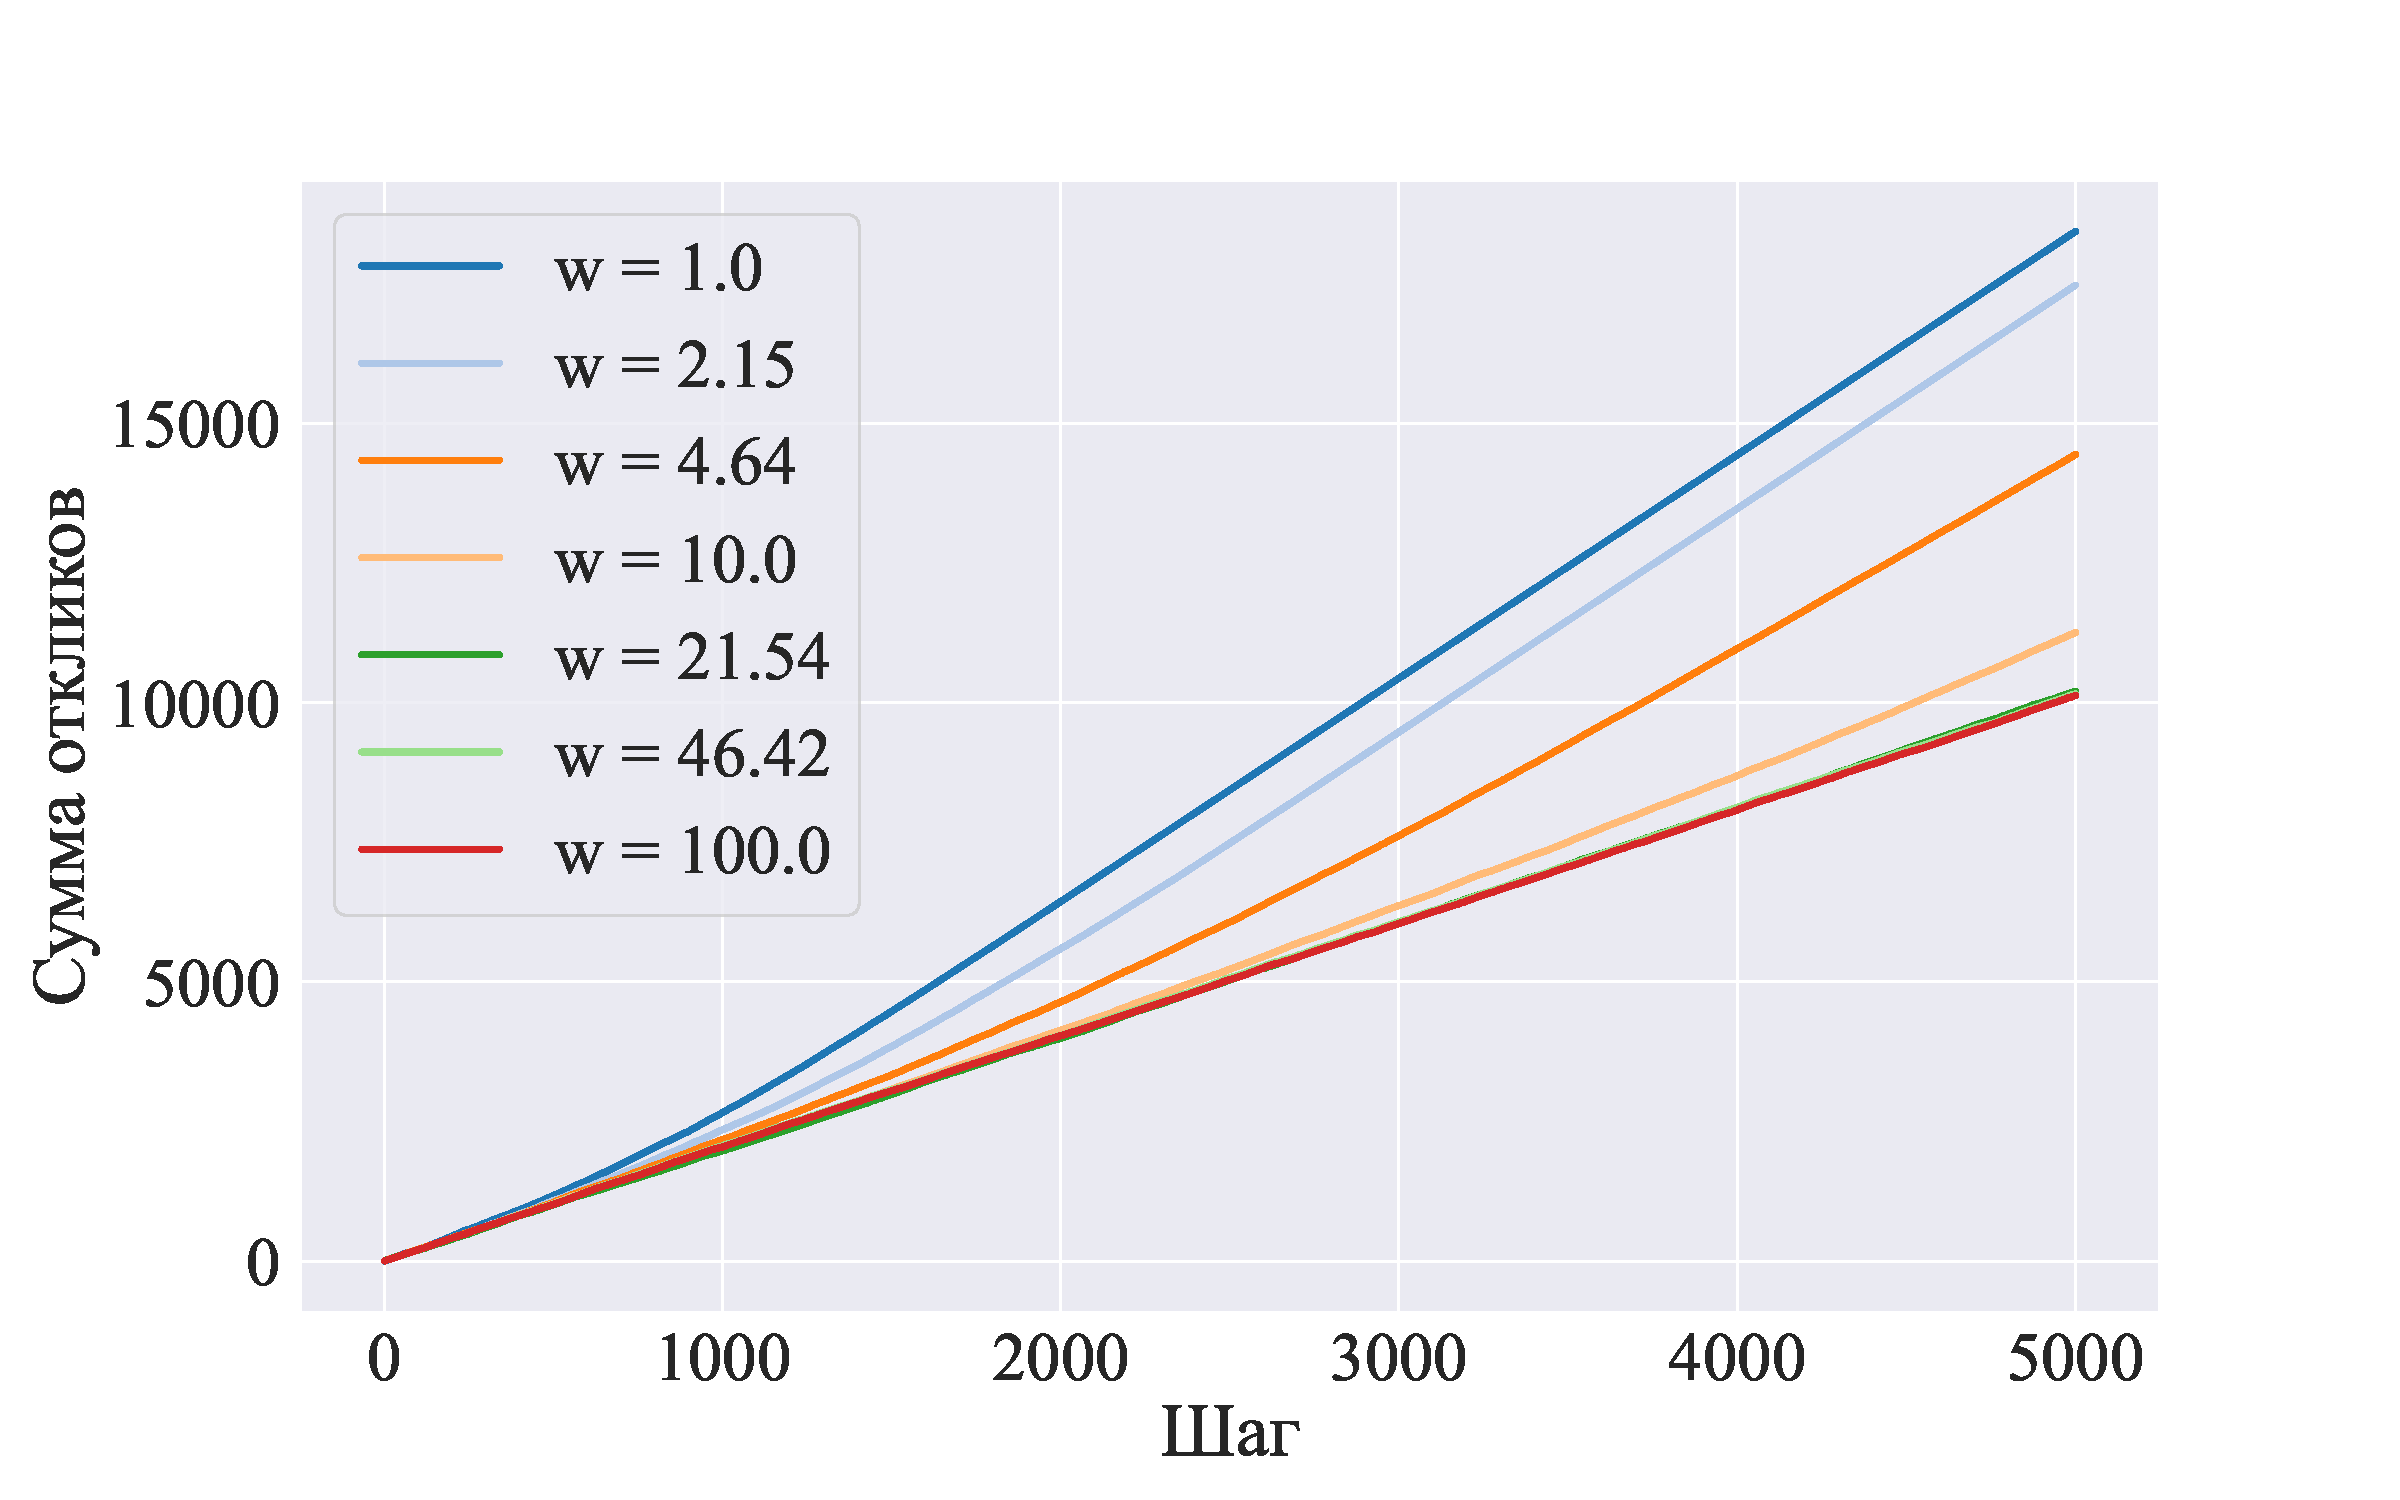
\includegraphics[width=6cm]{../rewards.pdf}
\end{center}
\end{columns}

\end{frame}
%------------------------------------------------------------------------------------
% \begin{frame}{Анализ ошибки}
% Распределение интереса от параметров шума $w, p$ после $2000$ итераций.
% \begin{columns}[c]
% \column{0.5\textwidth}
% \begin{center}
%   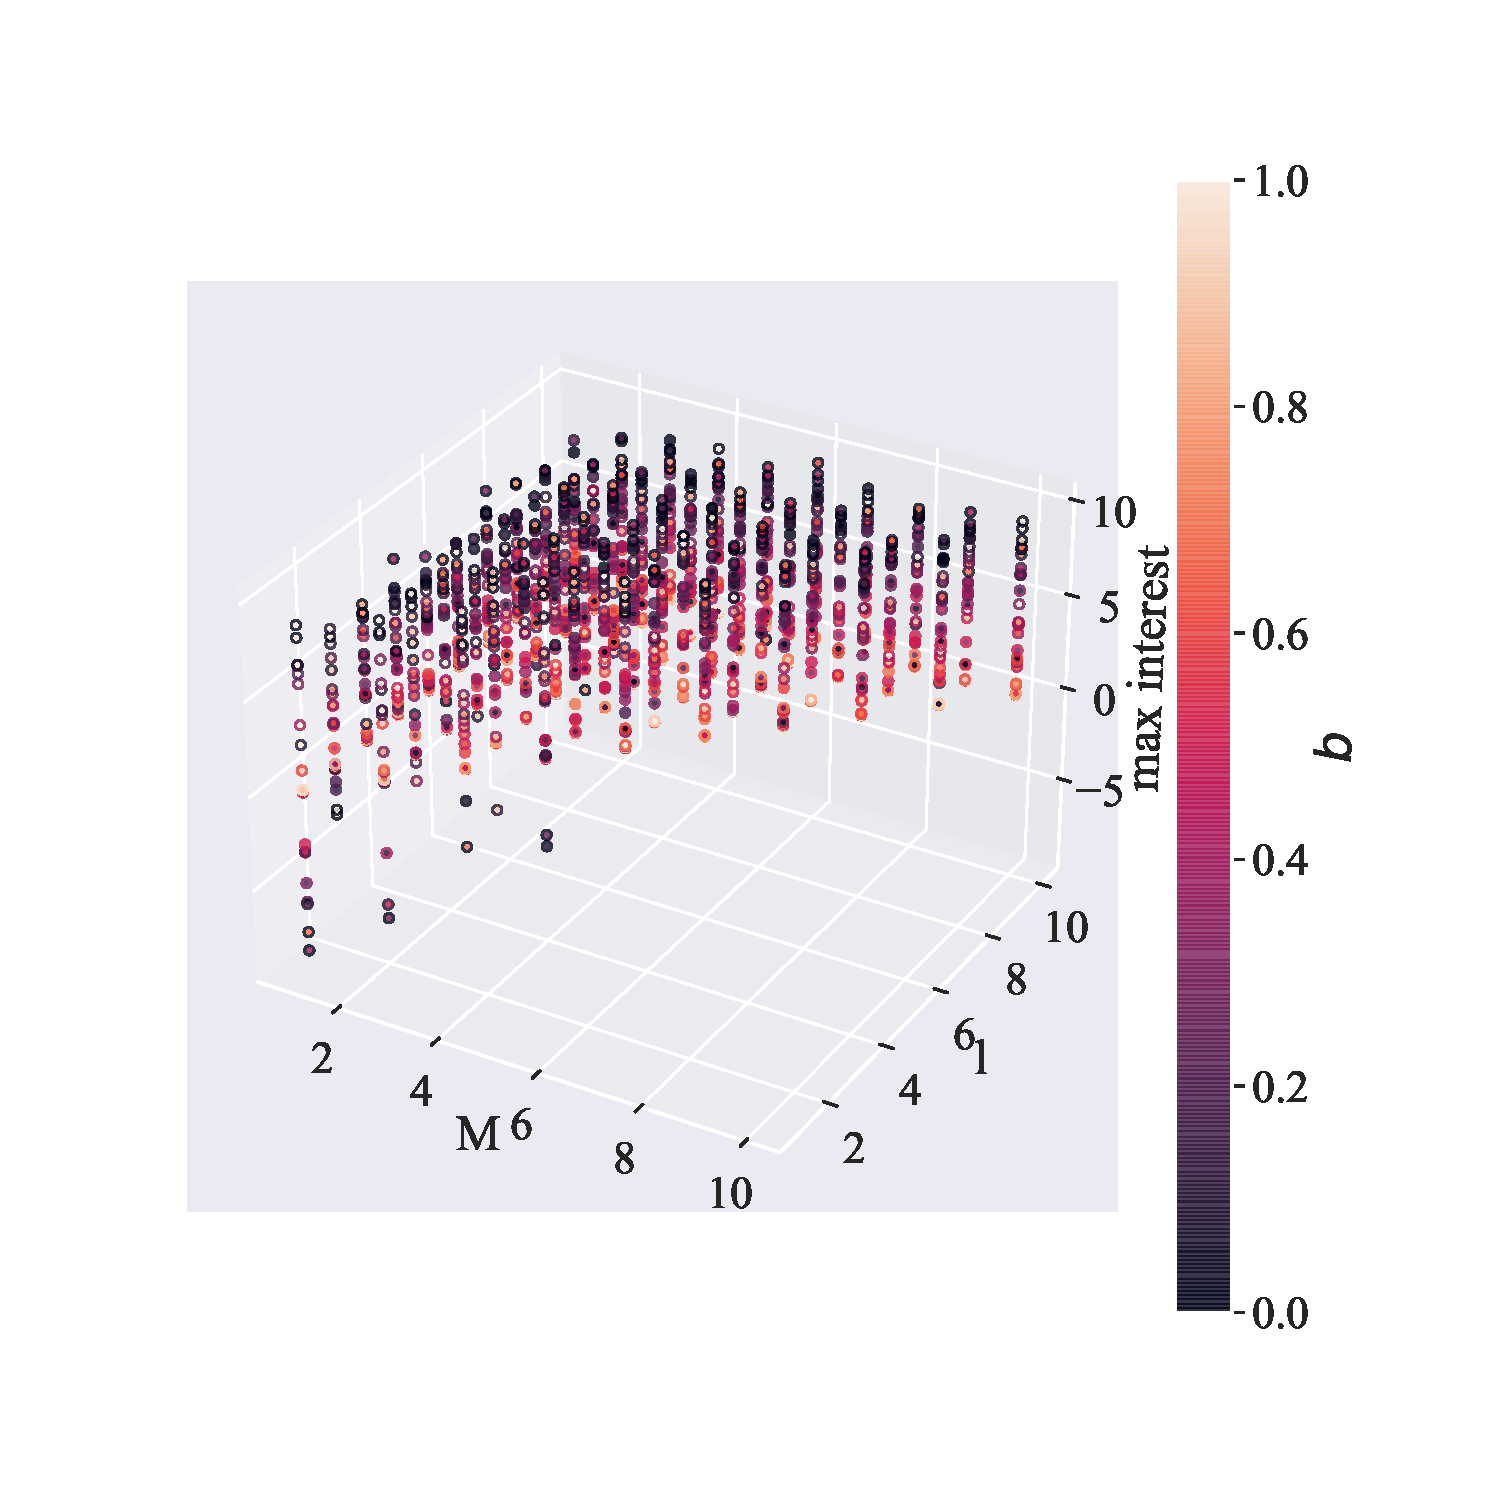
\includegraphics[width=6cm]{../3d_var_wp_max_interest.pdf}
% \end{center}
% \column{0.5\textwidth}
% \begin{center}
%   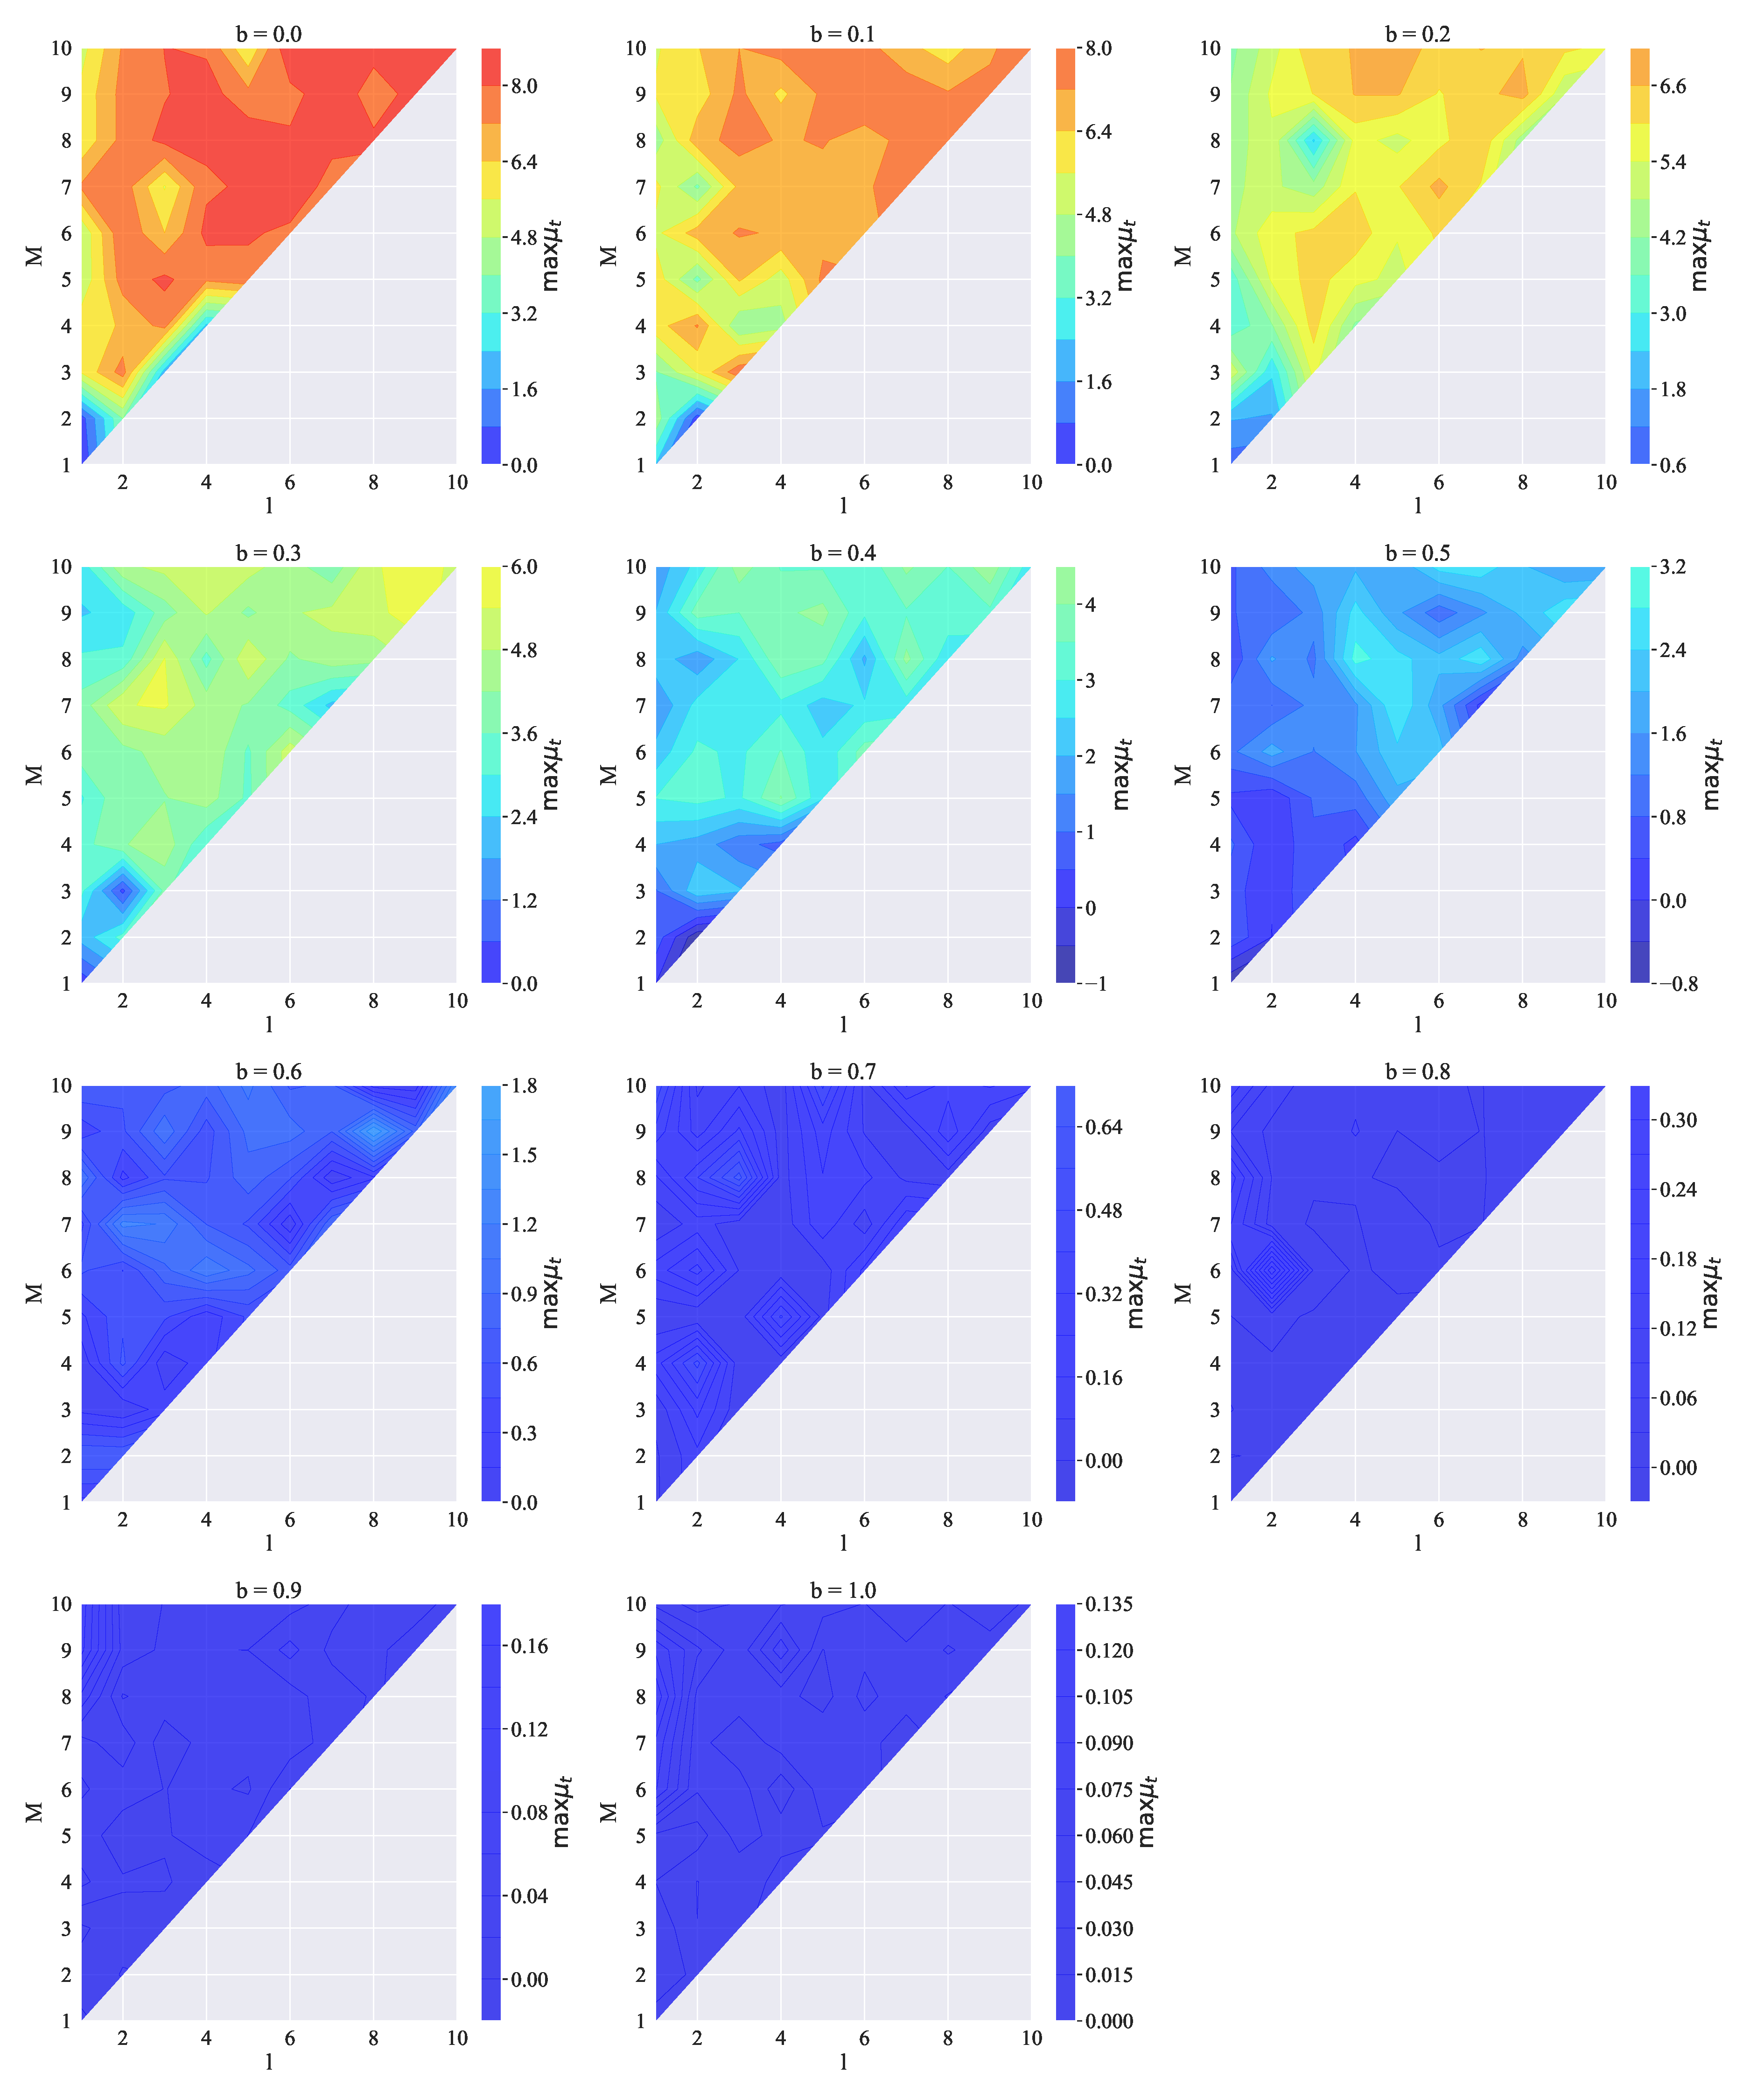
\includegraphics[width=6cm]{../countour_wp.pdf}
% \end{center}
% \end{columns}
% \end{frame}
%------------------------------------------------------------------------------------
\begin{frame}{Анализ ошибки}
\begin{columns}[T]
\column{0.5\textwidth}

Разброс нормы интереса
\begin{center}
  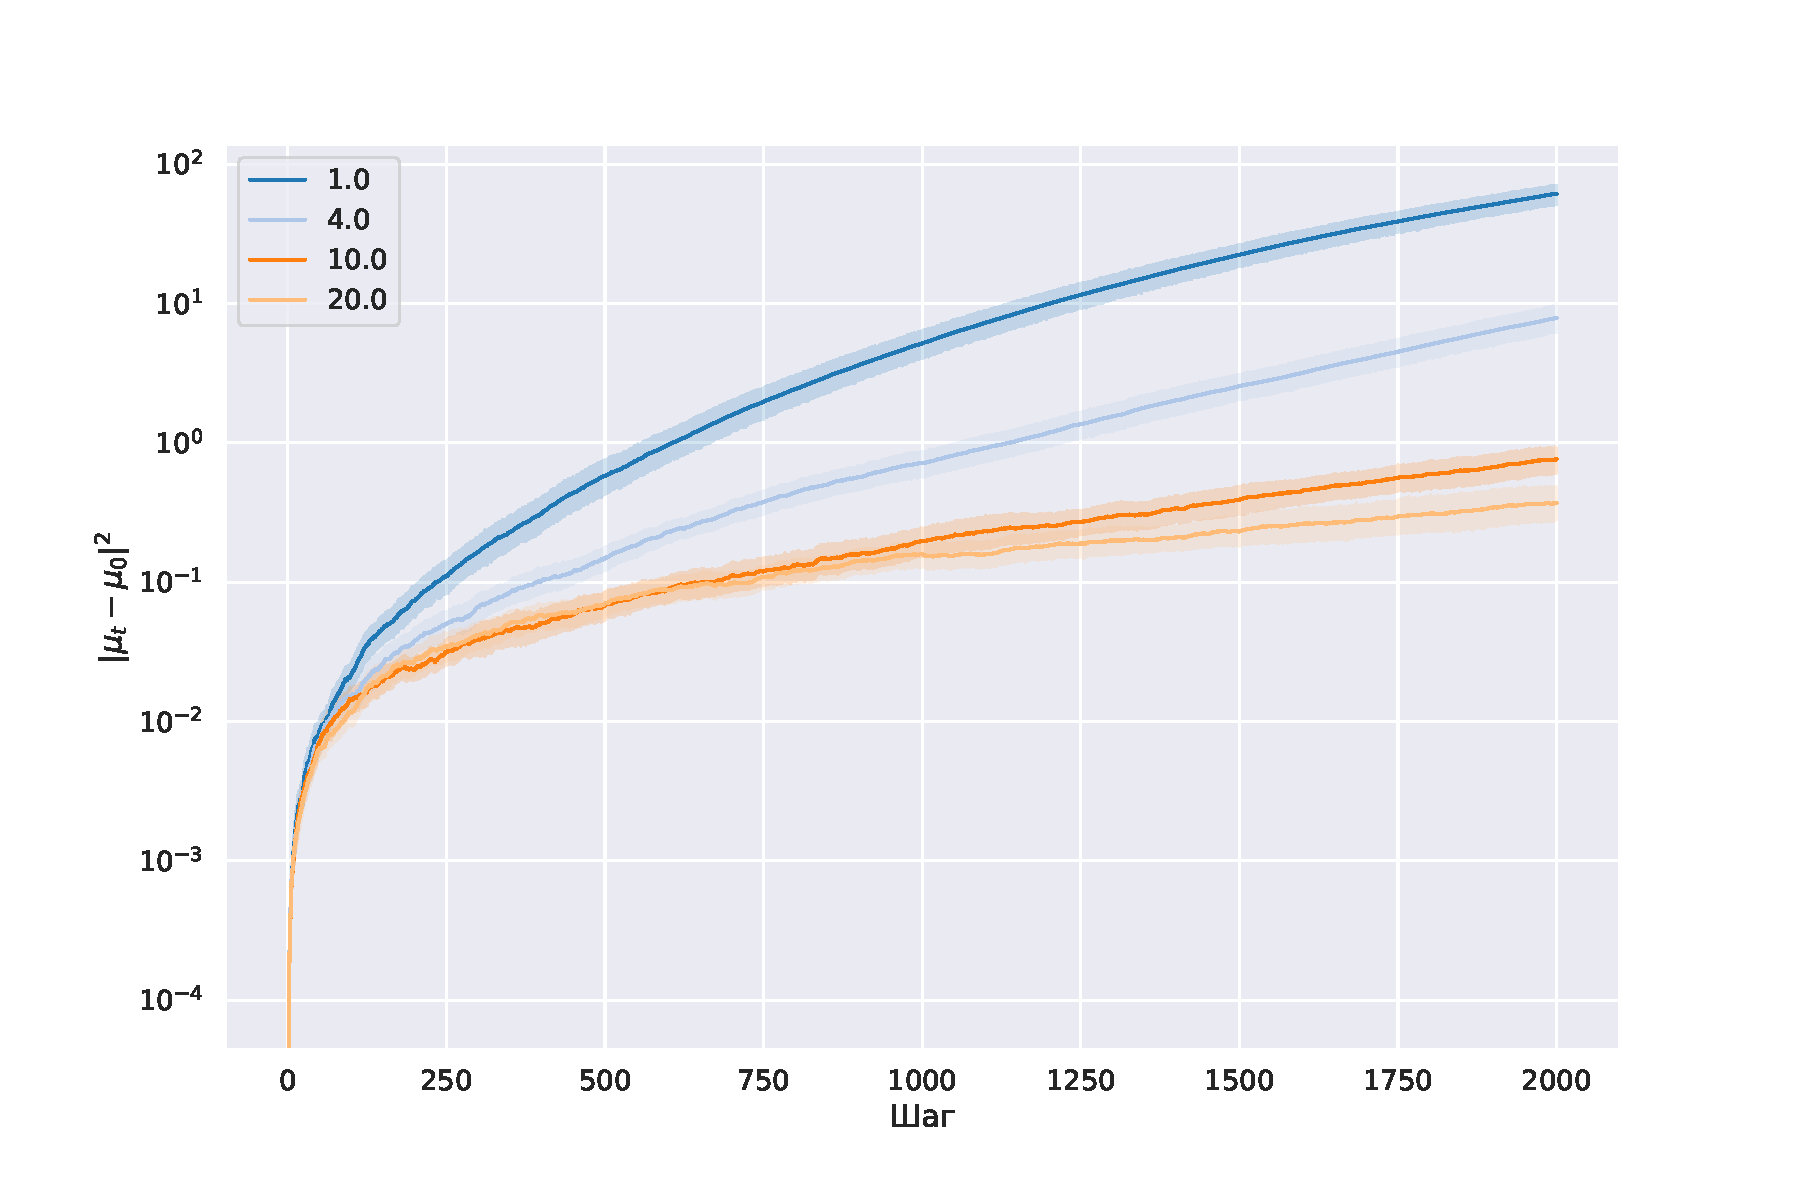
\includegraphics[width=6cm]{../var_norm_interest.pdf}
\end{center}
\column{0.5\textwidth}

Сравнивается MAB TS и рандомный алгоритм.
\begin{center}
  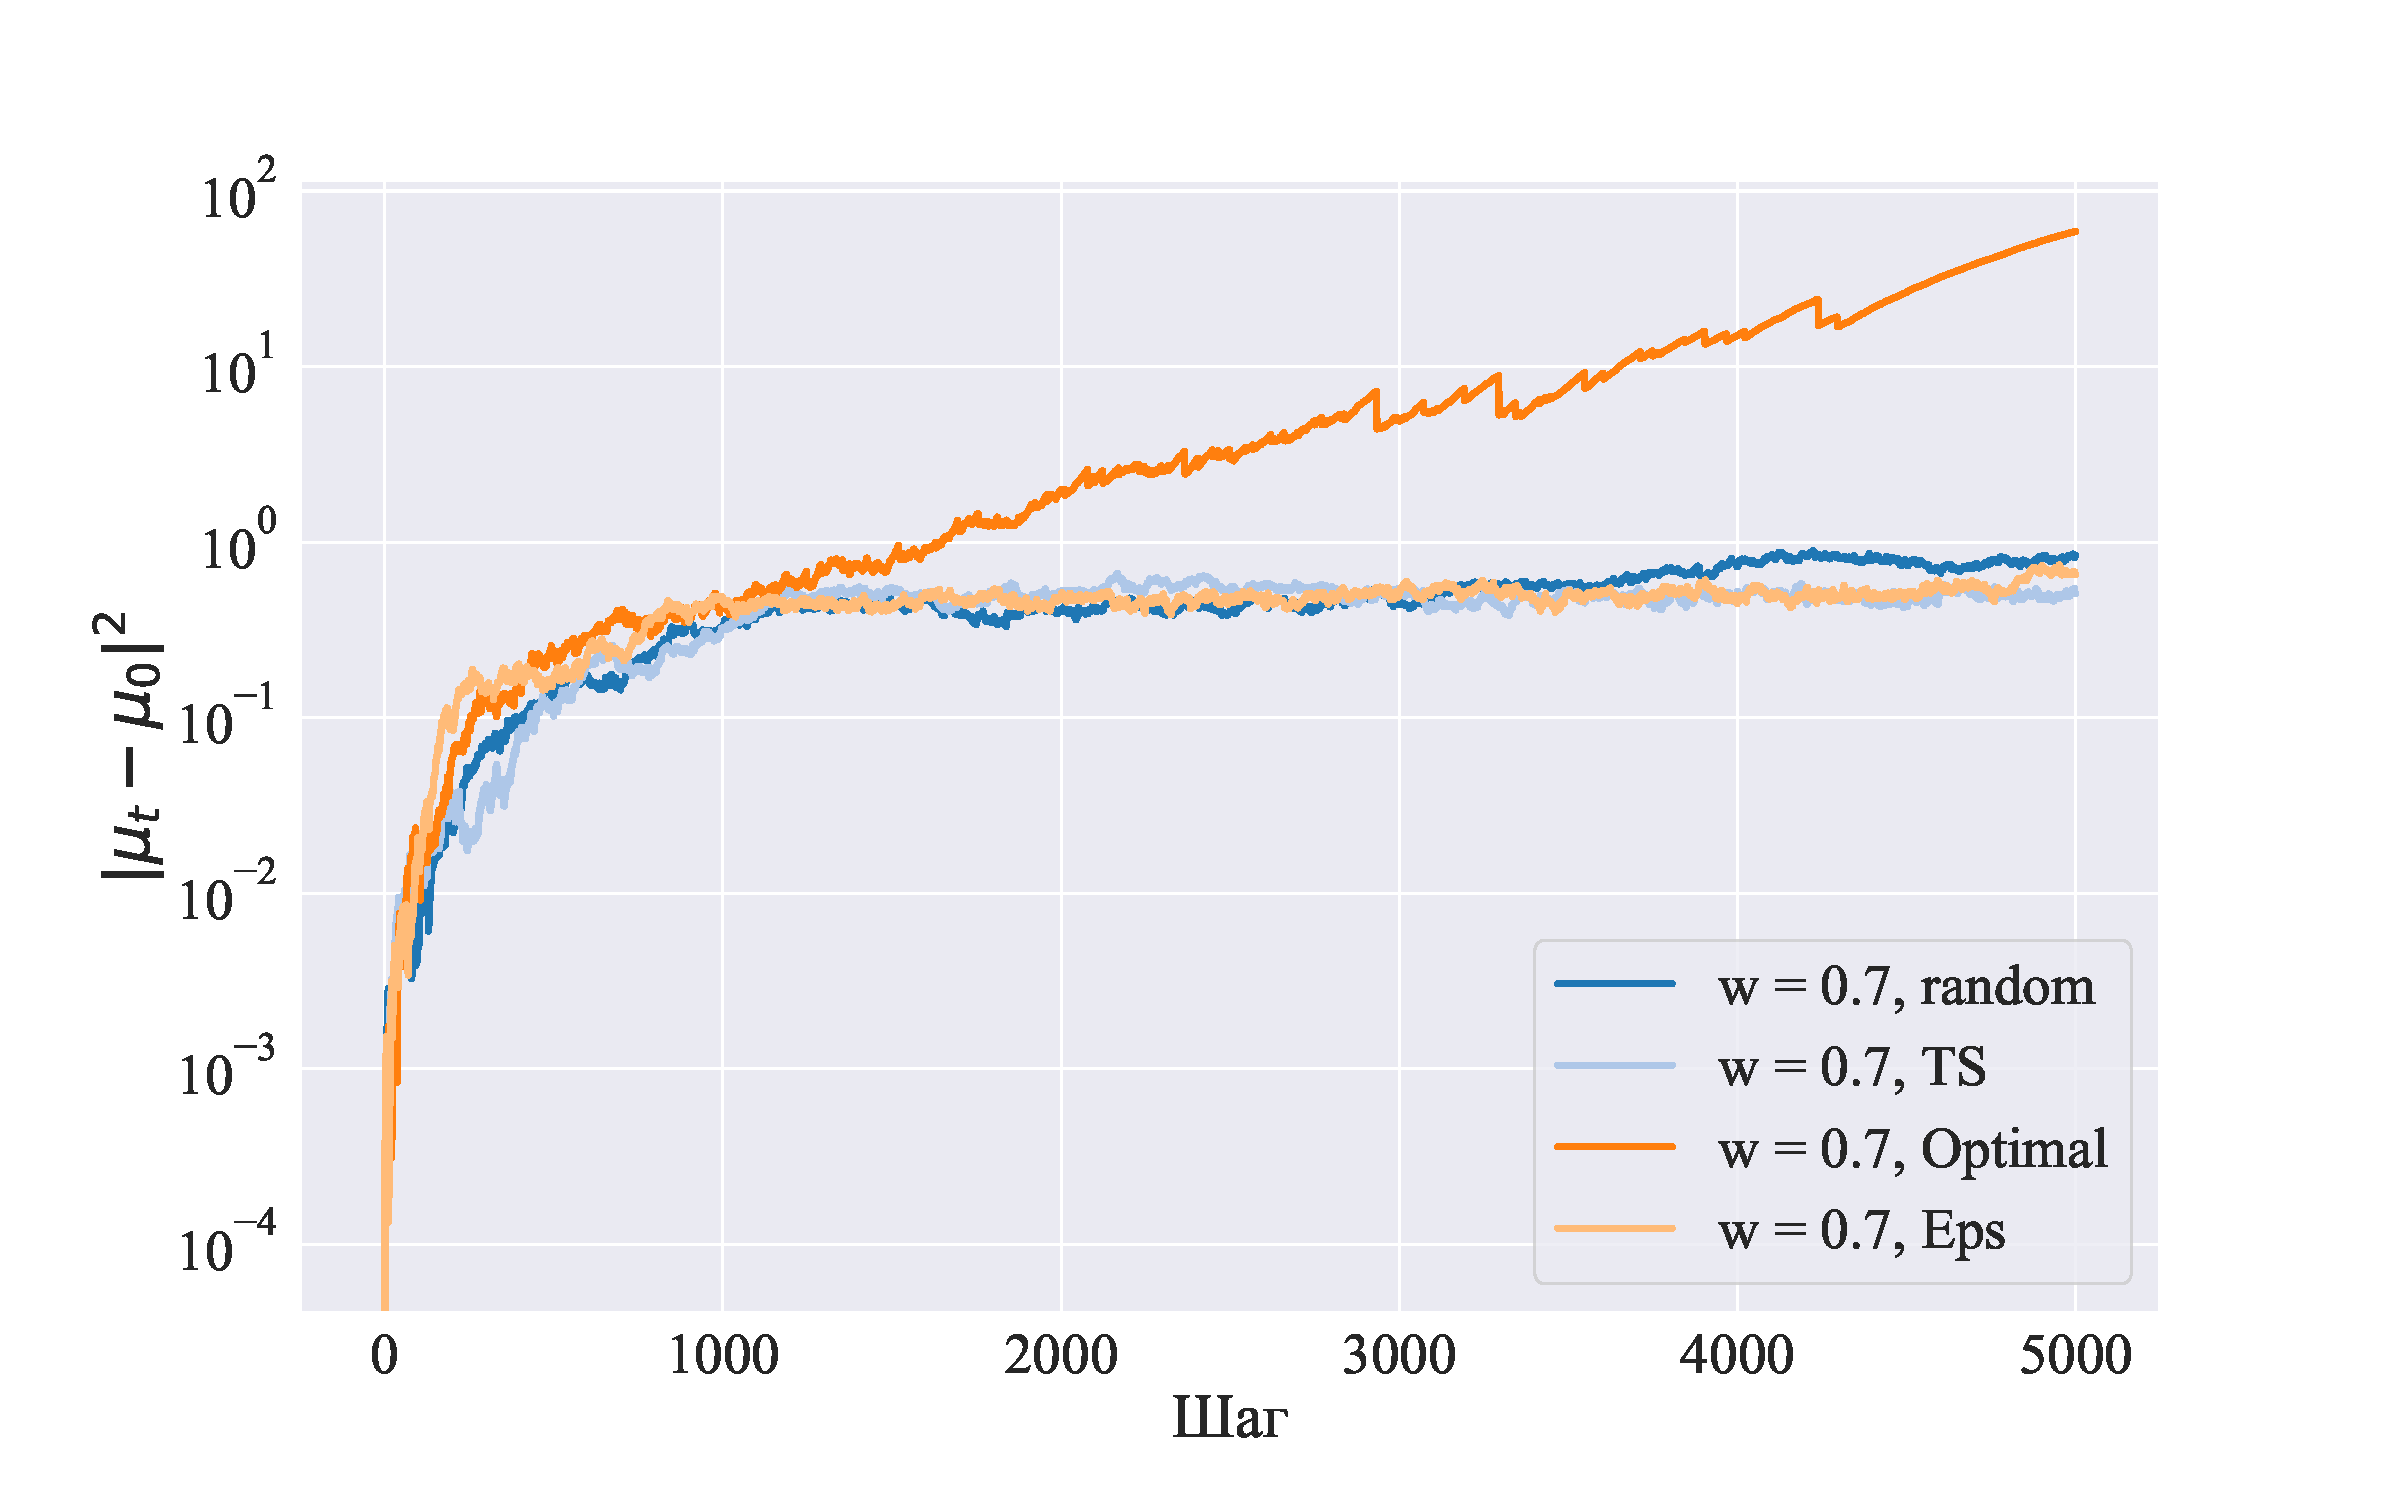
\includegraphics[width=6cm]{../compare_random_and_ts.pdf}
\end{center}
\end{columns}
\end{frame}
%----------------------------------------------------------------------------------------------------------
\begin{frame}{Заключение}
  \begin{itemize}
      \item Поставлена задача с учётом шума в ответах пользователя для рекомендательная системы использующей алгоритм TS
      \item Получено, что при любых парамeтрах аддитивного шума возникает петля  
      \item Показано, что утверждение подтверждается на эксперименте.
  \end{itemize}
\end{frame}
%----------------------------------------------------------------------------------------------------------
\end{document} 
